\documentclass[12pt, oneside]{article}
\usepackage[letterpaper, margin=1in, headsep=0.5in]{geometry}
\usepackage[english]{babel}
\usepackage[utf8]{inputenc}
\usepackage{amsmath}
\usepackage{amsfonts}
\usepackage{amssymb}
\usepackage{tikz}
\usetikzlibrary{quotes, angles}
\usepackage{graphicx}
%\usepackage{pgfplots}
%\pgfplotsset{width=10cm,compat=1.9}
%\usepgfplotslibrary{statistics}
%\usepackage{pgfplotstable}
%\usepackage{tkz-fct}
%\usepackage{venndiagram}

\usepackage{fancyhdr}
\pagestyle{fancy}
\fancyhf{}
\rhead{\thepage \\Name: \hspace{1.5in}.\\}
\lhead{BECA / Dr. Huson / 10.3 Geometry\\* 22 October 2018}

\renewcommand{\headrulewidth}{0pt}

\begin{document}
\subsection*{Monday modeling}
Show your work. For graphs, use a pencil and straight edge.
  \begin{enumerate}

\subsubsection*{Graphing linear functions}
\item Fill in the T-chart, plot the points, and draw the line.

    \begin{center} %4 quadrant regents grid w T-Chart
    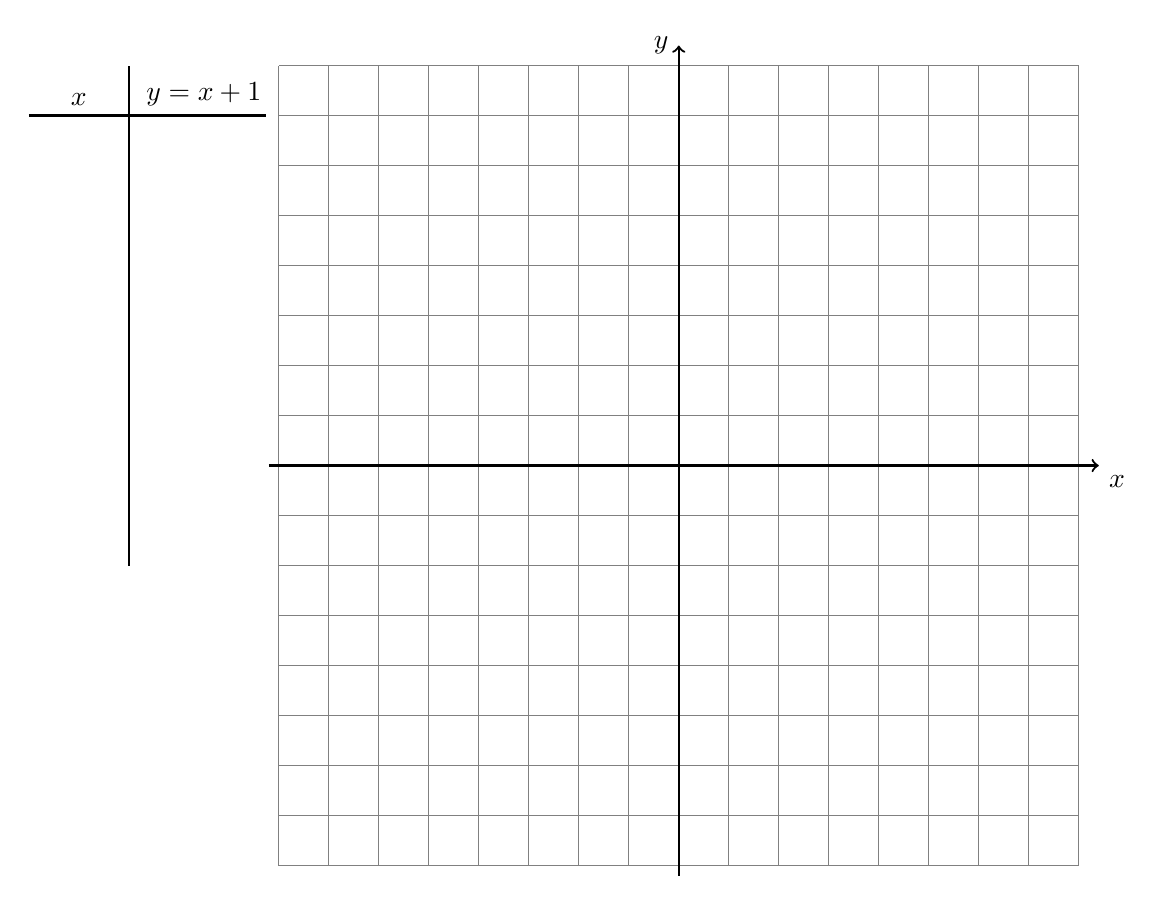
\begin{tikzpicture}[scale=.635]
      \draw [thick, -] (-11, -2)--(-11,8);
      \draw [thick, -] (-13,7)--(-8.25,7);
      \node at (-12,7) [above] {$x$};
      \node at (-9.5,7) [above] {$y=x+1$};
      \draw [help lines] (-8,-8) grid (8,8);
      \draw [thick, ->] (-8.2,0) -- (8.4,0) node [below right] {$x$};
      \draw [thick, ->] (0,-8.2)--(0,8.4) node [left] {$y$};
    \end{tikzpicture}
    \end{center}
Write down the slope and $y$-intercept of the line.\\[0.5cm]
$m=$\\[0.5cm]
$b=$\\[0.5cm]
Circle the row for the $y$-intercept.
\newpage

\item Find the slope of the function from the line differences.
    \begin{center}
      \begin{tabular}{|c|r|}
      \hline
      $x$ & $f(x)$\\
      \hline
      -1 & -3 \\
      \hline
      0 & -1 \\
      \hline
      1 & 1 \\
      \hline
      2 & 3 \\
      \hline
      3 & 5 \\
      \hline
      \end{tabular}
    \end{center}
Graph the function as a line over the domain $-1 \leq x \leq 3$.

\begin{center} %4 quadrant regents grid w T-Chart
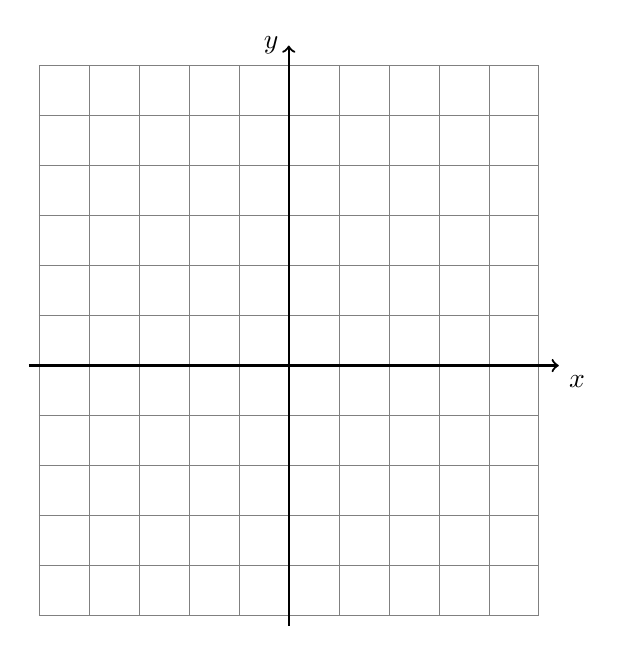
\begin{tikzpicture}[scale=.635]
  \draw [help lines] (-5,-5) grid (5,6);
  \draw [thick, ->] (-5.2,0) -- (5.4,0) node [below right] {$x$};
  \draw [thick, ->] (0,-5.2)--(0,6.4) node [left] {$y$};
\end{tikzpicture}
\end{center}


\subsubsection*{Simplify each expression (``Collect like terms")}

  \item $4x^2+3x -7 -2x^2-x+4$ \vspace{3cm}
  \item $3(a^2-2a +1) -2(a^2-a-4)$ \vspace{3cm}

\newpage

\item Show the line differences next to the table. Are the differences constant, i.e. a line with a slope?
    \begin{center}
      \begin{tabular}{|c|r|}
      \hline
      $x$ & $f(x)$\\
      \hline
      -1 & 8 \\
      \hline
      0 & 3 \\
      \hline
      1 & 0 \\
      \hline
      2 & -1 \\
      \hline
      3 & 0 \\
      \hline
      4 & 3 \\
      \hline
      5 & 8 \\
      \hline
      \end{tabular}
    \end{center}

Plot the points and graph the function as a curve over the domain $-1 \leq x \leq 5$.

\begin{center} %4 quadrant regents grid w T-Chart
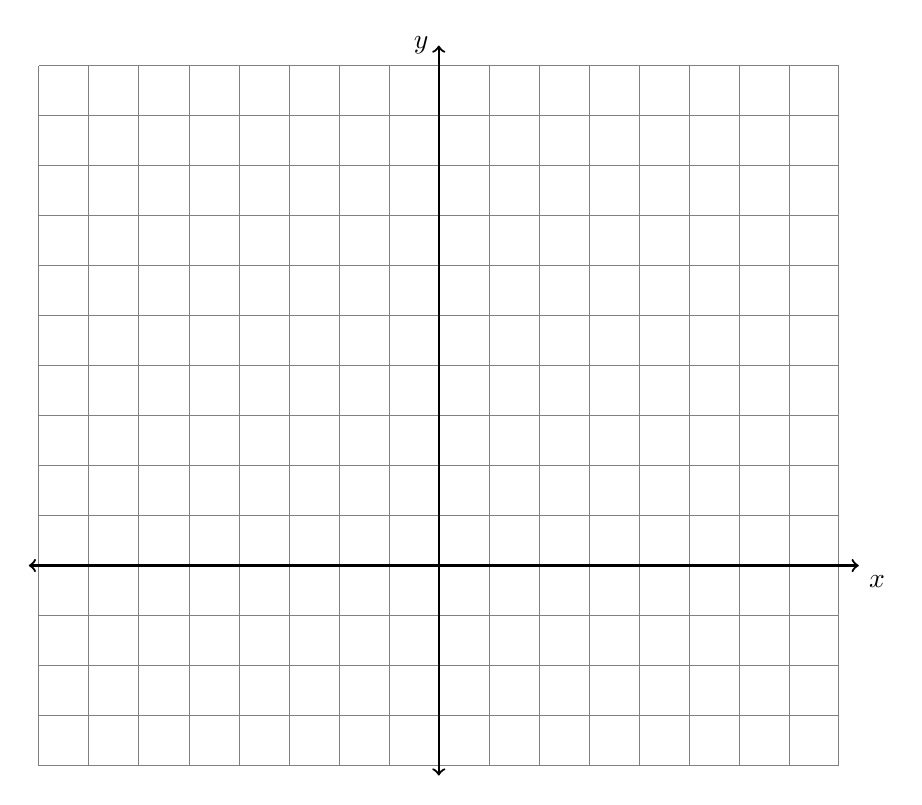
\begin{tikzpicture}[scale=.635]
  \draw [help lines] (-8,-4) grid (8,10);
  \draw [thick, <->] (-8.2,0) -- (8.4,0) node [below right] {$x$};
  \draw [thick, <->] (0,-4.2)--(0,10.4) node [left] {$y$};
\end{tikzpicture}
\end{center}

Mark the lowest point on the curve, the vertex, with a capital ``V".\\ \bigskip

Write down the two values for $x$ that make $f(x)=0$. \\[0.5cm]
a) $x=$ \hspace{3cm} b) $x=$

\newpage
%\subsubsection*{Solve equations}

Solve for the value of $x$.
\item   $8=x-3x$ \vspace{3cm}
\item   $\frac{1}{2}(x+7)=4x$ \vspace{4cm}
\item   $\frac{1}{3}x+2x-10=4$ \vspace{4cm}

\subsubsection*{Slope-intercept form}

What is the slope and $y$-intercept of each equation?
\item   $y=4x-2$ \vspace{1.5cm}
\item   $3x+y=5$ \vspace{3cm}


\newpage
\subsubsection*{Graphing linear functions}
Use pencil for graphs. Mark at least some of the values on each axis. Label each function with its name or equation.
\item Given the function $f(x)=-\frac{1}{2}x+4$.
\begin{enumerate}
    \item Write down the $y$-intercept. \bigskip
    \item Write down the slope of $f(x)$. \bigskip
    \item Draw the function $f(x)$ on the graph below.
    \item Label the intersection of $f(x)$ with the $x$-axis as the point $P$.
    \item Mark and label the point $Q (-2, 2)$.
    \item A second line, $g(x)$, is parallel to $f(x)$ and passes through point $Q$. Plot $g(x)$ on the graph.
    \item What is the $y$-intercept of $g(x)$? \bigskip
\end{enumerate}

\begin{center} %4 quadrant regents grid
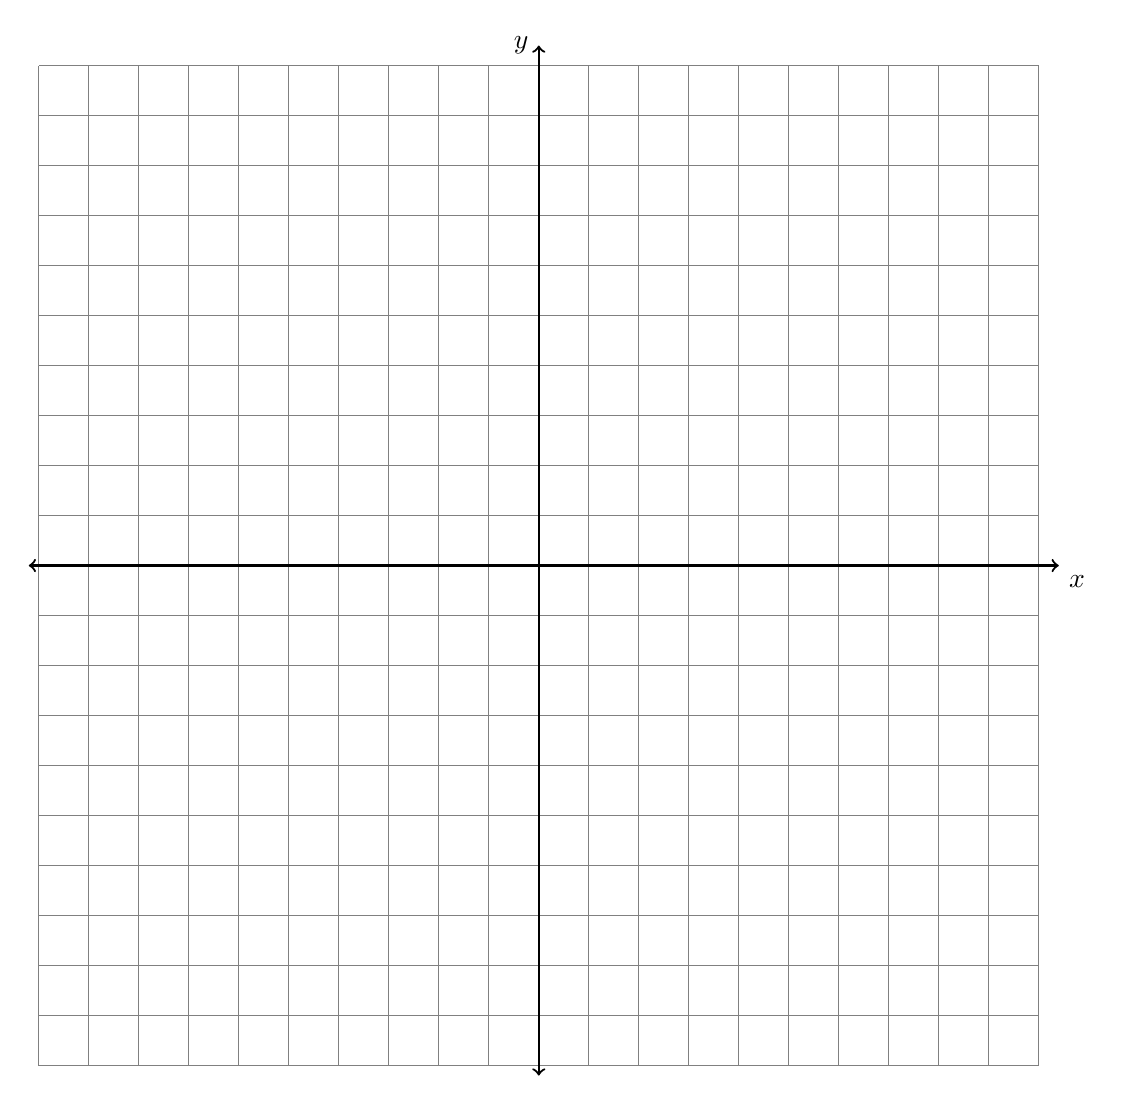
\begin{tikzpicture}[scale=0.635]
  \draw [help lines] (-10,-10) grid (10,10);
  \draw [thick, <->] (-10.2,0) -- (10.4,0) node [below right] {$x$};
  \draw [thick, <->] (0,-10.2)--(0,10.4) node [left] {$y$};
\end{tikzpicture}
\end{center}

\newpage
\item
  \begin{enumerate}
    \item Mark and label the point $P(4, 5)$ on the graph below.
    \item The line $L_1$ has a $y$-intercept of 3 and passes through point $P$. Graph $L_1$.
    \item What is the slope of line $L_1$? \vspace{2cm}
    \item What is the equation of line $L_1$? \vspace{2cm}
    \item A second line, $L_2$ has the equation $3x+4y=-8$. Plot $L_2$ on the graph.
    \item On the graph, mark the intersection of the two lines, $Q$, as an ordered pair.
  \end{enumerate}

  \begin{center} %4 quadrant regents grid
    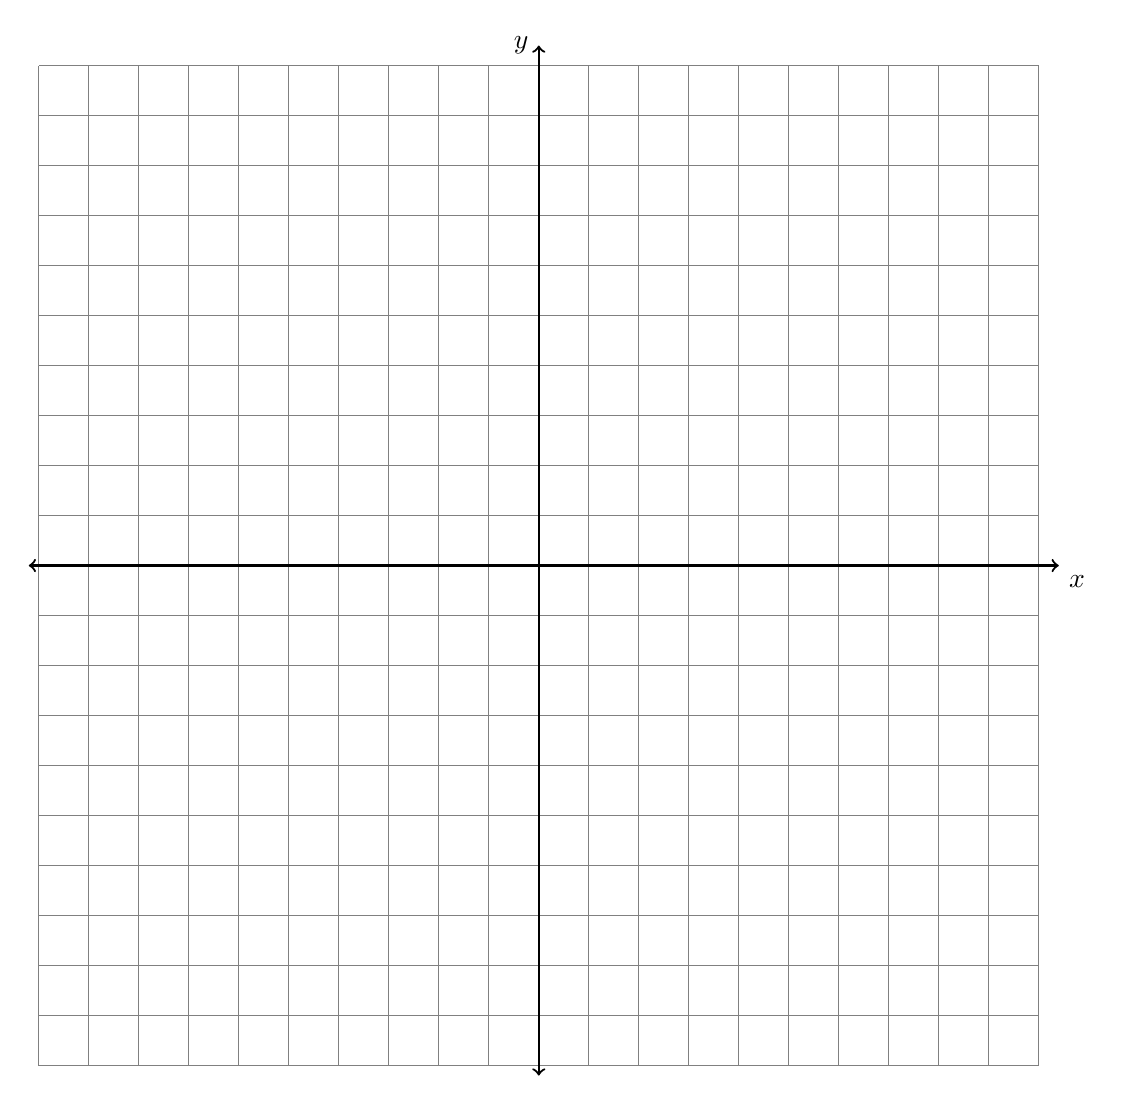
\begin{tikzpicture}[scale=0.635]
      \draw [help lines] (-10,-10) grid (10,10);
      \draw [thick, <->] (-10.2,0) -- (10.4,0) node [below right] {$x$};
      \draw [thick, <->] (0,-10.2)--(0,10.4) node [left] {$y$};
    \end{tikzpicture}
  \end{center}

\newpage
  \item Solve the system of equations by graphing each line and marking the intersection as an ordered pair.
    \[x+y=7\]
    \[y=3x+3\]

\begin{center} %4 quadrant regents grid
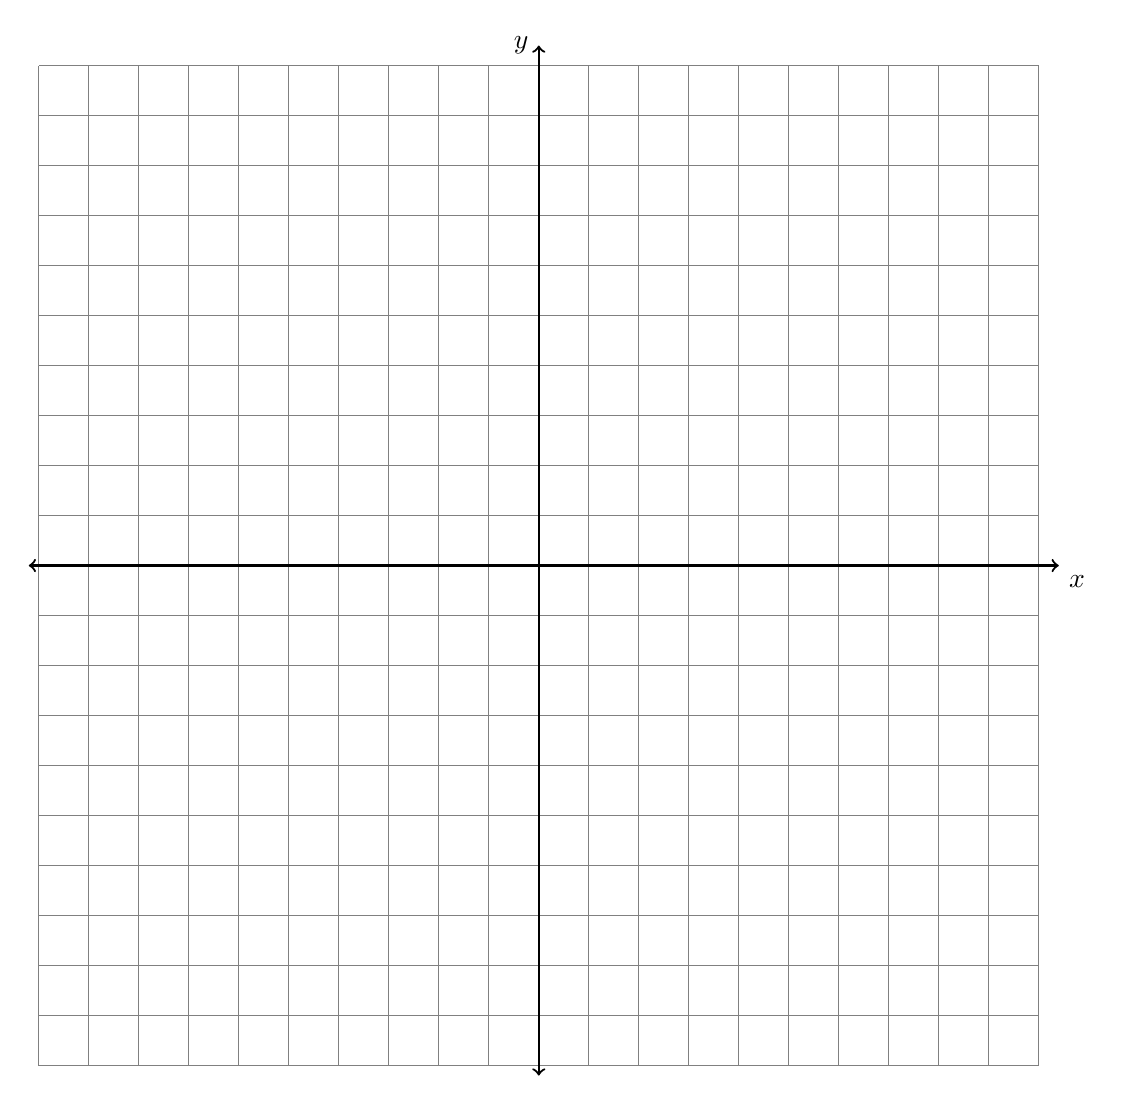
\begin{tikzpicture}[scale=0.635]
  \draw [help lines] (-10,-10) grid (10,10);
  \draw [thick, <->] (-10.2,0) -- (10.4,0) node [below right] {$x$};
  \draw [thick, <->] (0,-10.2)--(0,10.4) node [left] {$y$};
\end{tikzpicture}
\end{center}

\newpage
  Solve each system algebraically.
  \item
  $2x-4y=14$\\*
  $5x+4y=7$ \vspace{6cm}

  \item
  $2x-y=-7$\\*
  $3x+4y=17$  \vspace{6cm}


  \item Is the expression $2-\sqrt{5}$ rational, irrational, or neither? Explain.

\newpage
  \item Oceanside Bike Rental Shop charges a 17 dollar bike fee plus 6 dollars an hour for renting a bike. Jeffrey paid 53 dollars total. How many hours did he pay to have the bike checked out? \vspace{6cm}

  \item Three friends go bowling. The cost per person per game is \$5.30. The cost to rent shoes is \$2.50 per person. Their total cost is \$55.20. How many games did they play? \vspace{6cm}

  \item The admission fee at a small fair is \$1.50 for children and \$4.00 for adults. On a certain day, 40 people enter the fair and \$85.00 is collected. How many children and how many adults attended?

\newpage
  \subsubsection*{Function substitution}
  \item Given $f(x)=4x+7$. Simplify $f(2)$. \vspace{4cm}
  \item Given $\displaystyle f(x)=-\frac{(12+4x)}{11}$. Simplify $f(-3)$.

\newpage
\subsubsection*{Parallel and perpendicular linear equations}

  \item What is the equation of the line with a slope of 2 passing through the point $(0,1)$? \vspace{4cm}
  \item What is the equation of a line parallel to $y=-2x+1$ with a $y$-intercept of 4? \vspace{4cm}
  \item What is the slope of a line perpendicular to the line $x-2y=16$? \vspace{4cm}

\end{enumerate}
\end{document}
